%% This file is a portion of the source for Revised Edition 1.1 of
%% Operating Systems and Middleware: Supporting Controlled
%% Interaction, Copyright 2011 by Max Hailperin.  This work is
%% licensed under the Creative Commons Attribution-ShareAlike 3.0
%% Unported License. To view a copy of this license, visit
%% http://creativecommons.org/licenses/by-sa/3.0/ or send a letter to
%% Creative Commons, 171 Second Street, Suite 300, San Francisco,
%% California, 94105, USA.
\chapter{Security}
\label{security-chapter}

\section{Introduction}

I have addressed security issues in each preceding chapter because
security is a pervasive design issue, the same way performance is.
Just as one can't discuss virtual memory mechanisms or persistent
storage as though performance didn't exist and then devote a later
chapter solely to performance, it would have been wrong to treat
security as an add-on.  On the other hand, there has been such
sustained attention to security from so many talented researchers that
a rich, coherent body of security concepts has resulted, worthy of a
chapter of its own.

Section~\ref{security-objectives-and-principles-section} recapitulates
and amplifies on Chapter~\ref{intro-chapter}'s definition of security and
statement of security objectives.  It also lists a number of
high-level security principles, many of which were illustrated in
particular cases throughout the book.

Sections \ref{user-authentication-section} and
\ref{access-and-information-flow-controls-section} discuss the two
most well-developed areas of security technology: the authentication
of user identities and the provision of access control and
information-flow control to limit the authority of users.  The latter
topic builds on Chapter~\ref{processes-chapter}'s introduction to
protection.  (Another well-developed area of security technology,
cryptography, was addressed in Chapter~\ref{networking-chapter}.)

Section~\ref{viruses-and-worms-section} describes viruses and worms,
some of the most prevalent security threats, which fall largely
outside of the scope of conventional authentication and authorization
controls.  Because worms often propagate by exploiting buffer-overflow
vulnerabilities, I also describe this widespread form of vulnerability
in the same section.

Security measures are subject to imperfection, just like all other
human endeavors.  Sections \ref{security-assurance-section} and
\ref{security-monitoring-section} describe two responses to this
reality: (1) assurance techniques used to assess the quality of security
measures and (2) monitoring techniques used to collect information on
attacks, particularly any that are not thwarted.

Finally, Section~\ref{key-security-best-practices-section} closes the
book on a practical note by providing a summary of key security best
practices.  Many of these have already been mentioned in earlier
chapters or will be mentioned in the course of Sections
\ref{security-objectives-and-principles-section}--\ref{security-monitoring-section}.
However, by bringing all of them together in one place, I hope to
provide something of a checklist for your guidance.  After this
summary, the chapter ends with exercises, programming and exploration
projects, and notes.

\section{Security Objectives and
  Principles}\label{security-objectives-and-principles-section}

Security is best understood as one aspect of overall system quality.
Like quality in general, it refers to how well the system meets
the objectives of its owner or other primary stakeholders.  If you
think about all the factors that can stop a system from meeting those
objectives, it should be clear that quality stems from a combination
of proper design, implementation, and operation.  Similarly, security
spans all these areas.  Before examining what makes security different
from other aspects of quality, I would like to pin down the definition
of quality a bit more carefully.

A tempting first definition of a quality system is that it is one that
is designed, implemented, and operated so as to meet the objectives of
its owner.  However, this definition is somewhat unrealistic because
it fails to acknowledge that decisions, particularly regarding
design, need to be made without complete knowledge of how they will
affect the system's suitability.  Therefore, I would refine the definition
to say that a quality system is one that is designed, implemented, and
operated to reduce to an appropriate level the risk that it will
fail to meet the objectives of its owner.

A system's risk has been reduced to an appropriate level if it is
preferable to accept the remaining risk than to incur the costs of
further reducing the risk.  This definition makes risk management
sound like a straightforward economic calculation, like deciding
whether to continue paying high fire-insurance premiums for an old
warehouse or instead build a new, more fire-resistant warehouse.
Unfortunately, the decisions regarding system development and
operation are not so precisely calculable.

An insurance company has a good estimate of how likely the warehouse
is to burn down; the probability a computer system will fail to meet
objectives is far fuzzier.  In addition, the insurance company has a good
estimate of how large a loss would result from the fire, denominated
in dollars.  In contrast, the consequences of a low-quality computer
system may be difficult to predict, and in some cases may not be
adequately translatable into financial terms.  Consider, for example,
a computer system that is essential to national security.

Nonetheless, however imperfect the risk-management approach to
system quality may be, it provides the correct conceptual framework.
The management goal should be to expend resources in a way that
provides a commensurate reduction in risk.  This requires keeping in
view all three factors: cost, likelihood of failure, and consequences
of failure.  Moreover, all three factors may be manipulable.  For
example, rather than building a new warehouse, it may be preferable to
reduce the amount of material stored in the warehouse, thus reducing
the possible loss.  Similarly, rather than making a computer system
less likely to fail, it may be preferable to reduce reliance on the
system so that its failure would not be so significant.  That
reliance may be reduced through the use of redundant computer systems
as well as through the use of noncomputerized systems.

Having provided this background on quality in general, I can define
system security similarly.  A system is secure if it is designed,
implemented, and operated so as to reduce to an appropriate level the
risk that it will fail to meet the objectives of its owner, even in
the face of adversaries.  An \vocab{adversary} is someone with
objectives so contrary to those of the owner as to strive to make the
system fail.

One mildly interesting consequence of this definition is that security
is irrelevant for low-quality systems, because they will fail to meet
their owners' objectives even without intervention by adversaries.
However, the more interesting consequence is that the risk-management
approach to system quality needs to be extended to include the actions
of adversaries.

A secure system need not be impervious to attack by adversaries.  In
fact, it need not even be especially difficult for adversaries to
interfere with.  Instead, what is needed is that the likelihood an
adversary will choose to mount an attack, the likelihood that the
attack will succeed, and the damage likely to be done to the system
owner's objectives by a successful attack all combine to produce an
appropriate level of risk relative to the cost of available
countermeasures.

Generally, an acceptable level of risk will not be achievable if the
system offers no resistance to attack.  However, at some point further
reduction in the system's vulnerability will be a less appropriate
risk-management approach than reducing the threats the system faces
and the consequences of a successful attack.

Some of these risk-management actions may be nontechnical.  For
example, if the organization can avoid creating disgruntled employees,
its systems will not face such severe threats, independent of how
vulnerable they are.  As another example, a company might choose to
accept the cost of repeated data entry rather than store its
customers' credit-card numbers online.  Doing so will both reduce
threats (because adversaries will have less motivation to break into
the system) and reduce the consequences of successful attacks (because
the company will lose less customer goodwill).

However, it would be wrong to equate technical efforts with only the
reduction of vulnerabilities and assume that all efforts to reduce
threats or the consequences of failure are nontechnical in nature.  In
fact, one of the most active technical areas today is the monitoring
of systems' operation; I discuss this in
Section~\ref{security-monitoring-section}.  This monitoring does
nothing to reduce a system's inherent vulnerability.  However, it both
deters adversaries (especially adversaries internal to the
organization), thereby reducing threats, and allows rapid-response
incident-handling teams to quickly and efficiently get systems
operational again after attacks, thereby reducing losses.

So, what might the owner's objectives be that an adversary could seek
to thwart?  There is no end to the specific objectives an owner might
have.  However, there are four broad classes of objectives that
commonly arise in discussions of security:
\begin{itemize}
\item The owner may wish to maintain the \vocab{confidentiality} of
  information stored in the computer system.  That is, the information
  should not be disclosed to any person who has not been authorized to
  receive it.
\item The owner may wish to maintain the \vocab{integrity} of
  information stored in the computer system.  That is, the information
  should not be modified or deleted by any person who has not been
  authorized to do so.
\item The owner may wish to preserve the \vocab{availability} of the
  services provided by the computer system.  That is, persons
  authorized to use the system should be able to do so without
  interference from adversaries.  The adversaries
  should not be able to cause a \vocab{denial of service}.
\item The owner may wish to ensure \vocab{accountability}.  That is,
  it should be possible to determine how users have chosen to exercise
  their authority, so that they can be held responsible for the
  discretionary choices they made within the limits set by the
  security controls.
\end{itemize}

All four of these objectives have a common prerequisite, user
\vocab{authentication}.  That is, the system must verify that each
user is correctly identified.  Without reliable user identities, there
is no way the system can enforce a restriction on which users can
retrieve or modify information and no way it can keep records of who
has done what.  Even availability relies on authentication, because
without a way to determine whether a user is a bona fide system
administrator, there is no way to control the use of commands that
shut the system down.

To increase the chance that these objectives are achieved, system
designers have found it useful to have a guiding set of principles.
These are more specific than the overall risk-management perspective
sketched earlier, but less specific than individual technical
measures.  Most of these principles came to prominence in a 1975 paper
by Saltzer and Schroeder, though they date back yet further.  The
following list largely echoes Saltzer
and Schroeder's:
\begin{description}
\item[Economy of mechanism:]
Simple designs that consistently use a small
number of general mechanisms are more likely to be secure.  An
example would be Chapter~\ref{transactions-chapter}'s point that a
general-purpose transaction-processing infrastructure is more likely
to be secure than individual ad hoc mechanisms for atomicity.
\item[Fail-safe (and fail-noisy) defaults:]
A security system should be
designed to withhold access by default.  If anything goes wrong in the
granting of authority, the result will be too little authority, rather
than too much.  This makes the problem more likely to be fixed,
because legitimate users will complain.  An
example from Chapter~\ref{processes-chapter} is Microsoft's mechanism
for resolving conflicts between ACL entries. That mechanism governs the case when one entry says to allow a
permission and another says to deny it.  The kernel itself is not
fail-safe, because it gives precedence to whichever entry is listed
first.  However, the higher-level API used by the GUI is fail-safe,
because it always gives precedence to denying permission.
\item[Complete mediation:]
Ideally, every access should be checked for
authority.  Processes should not be allowed to continue accessing a
resource just because authority was checked at some earlier point.  An
example from Chapter~\ref{processes-chapter} is the change IBM made in
deriving the AS/400 design from the System/38.  The original design
used ACLs to decide whether to grant capabilities, but then allowed
the capabilities to be retained and used without any further reference
to the ACLs.  The revised design causes the ACLs' record of
authorization to be checked more consistently.
\item[Open design:]
The only secret parts of the security mechanism should be
cryptographic keys and passwords.  The design should be inspected by
as many parties as possible to increase the chance of a weakness
coming to light.  An example would be
Chapter~\ref{networking-chapter}'s description of openly standardized
cryptographic algorithms.  In particular, that chapter mentioned that
the MD5 algorithm was found to be weak.  I would not have been
able to give you that warning without the public scrutiny MD5 has
received.
\item[Separation of privilege:]
No one individual should be authorized to
carry out any particularly sensitive task.  Instead, the system should
be designed so that two authorized users need to collaborate.  Among
other benefits, this defends against the corruption of persons in
positions of authority.
\item[Least privilege:]
Each process should operate with only the authority
it needs so that even if an adversary makes something go wrong in the
process's execution, there will be many kinds of damage it can't do.
In Chapter~\ref{synchronization-chapter}, I described a case where
adversaries exploited a Time Of Check To Time Of Use (TOCTTOU) vulnerability to trick a mail delivery
program into writing into sensitive files.  I highlighted the failure
to use proper synchronization, resulting in the vulnerable race
condition.  However, I could equally well point to that mail program
as a failure to honor the principle of least privilege.  The mail
program needed authority only to write in each user's mail file, not
authority to write in all files whatsoever.  Because UNIX provided no
easy way to grant it just the requisite authority, it was given way
too much, and hence its vulnerability was rendered far more dangerous.
\item[Psychological acceptability:]
All security mechanisms must have
sufficiently well-designed user interfaces that they will be used
correctly.  An example is the graphical user interface Microsoft
Windows provides for ACLs, as shown in
Chapter~\ref{processes-chapter}.  As I pointed out there, the user
interface design includes such features as hiding unnecessary
complexity.
\item[Work factor:]
Just as you reason about the cost and benefit of security
countermeasures, you should reason about your adversaries' cost/benefit
trade-offs.  You should make sure that breaking into your systems takes
more time and trouble than it is worth.  An example would be the
discussion of cryptographic key length in
Chapter~\ref{networking-chapter}.  Keys are not completely secure, in
that they can be figured out with sufficient trial and error.
However, the usual key lengths are such that adversaries will not have
the resources necessary to find the keys in this way.
\item[Compromise recording:]
If the system's security is breached,
information about the breach should be recorded in a tamper-proof
fashion.  This allows an appropriate technical and legal response to
be mounted.  An important example of this principle, described in
Chapter~\ref{networking-chapter}, is the use of network intrusion
detection systems.
\item[Defense in depth:]
An adversary should need to penetrate multiple
independent defenses to be able to compromise a system's functioning.
For example, Chapter~\ref{networking-chapter} suggested the use of
multiple firewalls, such as hardware firewalls at the organizational
and workgroup perimeters and a software firewall on each desktop
machine.
\item[Alignment of authority and control:]
The same person should control
what a process will do and supply the authorization credentials for
the process's action.  In Chapter~\ref{processes-chapter}, I described
the risk of Trojan horse programs, which combine their executors'
authority with their authors' control, and setuid programs, which may
combine their executors' control with their authors' authority.  Many
network server programs have problems similar to setuid programs, in
that they allow anonymous individuals elsewhere on the Internet some
degree of control over their actions while using a local user's
authority.
\item[Physical security:]
The system's owner should control physical access to computer equipment and
unencrypted data.
An example from Chapter~\ref{persistence-chapter} is that disk drives
must be protected from physical theft.
Otherwise, confidentiality cannot be ensured.  As another example, I
once visited an organization that was in the business of printing and mailing out lots of checks
to individuals.  Much to my shock, their computer room was wide open.
Here the threat is to integrity rather than confidentiality.  An
adversary could exploit physical access to change the list of
recipients for the checks---an attractive proposition.
\end{description}

Before leaving this section of generalities and diving into technical
specifics, I want to return to the topic of adversaries.  Adversaries
can be outside your organization, but they can also be inside.  Either
way, they may exploit technical vulnerabilities, misuse authority they
have been granted, or engage in \vocab{social engineering}, that is,
tricking others who may have greater authority into cooperating. For
this reason, I generally use the word adversary rather than such
alternative terms as intruder and cracker.  The word \vocab{intruder} implies
an external adversary, and \vocab{cracker} implies one who uses technical
means.  The largest danger is that if you use one of these terms, you
may blind yourself to significant threats.  For example, protecting
your organization's network perimeter may be a fine defense against
intruders---but not against all adversaries.

Occasionally I will call an adversary an intruder or cracker, when
appropriate.  However, I will never call one a hacker, contrary
to what has become common usage.  Decades before crackers co-opted the
word, it meant someone who had a deep, creative relationship with
systems.  Many of the technologies taken for granted today were
developed by people who described themselves as hackers.  Today, I
would no longer dare call such a person a hacker outside a
knowledgeable circle of old-timers, for fear of being misunderstood.
However, just because I no longer use the word in
its traditional sense does not mean I would use it for
crackers.

\section{User Authentication}\label{user-authentication-section}

You are probably most familiar with user authentication in a very basic
form: logging into a computer system using a password at the start of
a session of usage.  This authentication mechanism suffers from
several potentially serious weaknesses:
\begin{itemize}
\item Because the authentication takes place only at the beginning of
  the session, the computer system at best knows who was seated at the
  keyboard then.  No attempt is made to notice whether you have walked
  away and someone else has taken your place.
\item Because you identify yourself using something intangible (your
  knowledge of a password), there is nothing to discourage you from
  sharing it with someone else.  You wouldn't need to give up your own
  knowledge to let someone else also have it.
\item Similarly, someone can steal the password without depriving you
  of it, and hence without drawing attention to themselves.  As an
  example, if you have written the password down, the adversary can
  copy it yet leave you your copy.
\item Because the same password is used each time you log in, anyone
  who observes you using it can then reuse it.  This is true whether
  they physically observe your typing (known as \vocab{shoulder
  surfing}) or use technical means to capture the password, either
  with covert software on the computer where you are typing (a
  \vocab{keylogger}) or with a network packet capture program (a
  \vocab{sniffer}).  The use of network encryption prevents sniffing but
  not the other techniques.
\item Either the password is easy for you to remember, in which case
  it is also probably easy for an adversary to guess, or you wrote it
  down, thereby exposing it.
\end{itemize}
In addition, there are several other pitfalls that, though not
unavoidable, are common in actual password systems:
\begin{itemize}
\item
If you type in your password without the computer system having first
authenticated itself to you, then you could fall prey to a
\vocabing{spoof} attack, in which the adversary sets up a fake system
to capture passwords and then presents them to the real system.
\item
If the system checks your password by comparing it with a copy it has
stored, then any exposure of its storage would reveal your password
and probably many others.
\item
If you have to choose your own passwords for many different systems
and are like most people, you will use the same password for several
different systems.  This means any weakness in the security of one
system, such as the use of stored passwords, will spread to the others.
\end{itemize}

With such a long list of weaknesses, you can be sure that security
specialists have devised other means of authentication.  I will
discuss those in Section~\ref{two-factor-section}.  Nonetheless, I would first like to explain how you can make the best of password
authentication because it is still widely used.  I will start with the most avoidable weaknesses, which are
those listed most recently: spoofing, storing passwords, and choosing the
same passwords for several systems.

\subsection{Password Capture Using Spoofing and Phishing}

One form of spoofing attack is to write a program that puts the correct
image on the screen to look like a logged-out system prompting for
username and password.  Thus, when someone comes up to the computer
and sees what looks like a login screen, they will enter their
information, only to have it recorded by the program.  The program can
avoid detection by displaying a realistic error message and then
logging itself out, returning to the genuine login window.  To defend
against this version of a spoofing attack, there needs to be something
the genuine login window can do to authenticate itself to users that
no other program could do.  Microsoft Windows can be configured to
take this approach by requiring users to press the CTRL+ALT+DEL
key combination at the start of a login.  The reason Microsoft chose
this combination
is that Windows allows programmers to draw anything at all to the
screen and to respond to any other key combination, but not
that one particular key combination.  Thus, so long as Windows
is running, you can be sure that CTRL+ALT+DEL is being responded
to by Windows itself, not by a spoofing program.  The one hitch is that a
spoofer could have installed software that runs without Windows.  To defend
against that, you would need to use physical security, which is
important for other reasons anyhow.

Another style of spoofing has become more problematic lately.  A web
site may be set up to look like a password-protected site, but really
be in the business of capturing the passwords.  Users can be directed
to the fake site using sophisticated network manipulations, but more
commonly they are simply tricked into accessing it using a misleading
email message, a technique known as \vocabing{phish}.  One important
countermeasure in this case is user education.  Users need to be much
less credulous of emails they receive.

However, there is also a technical dimension to the problem of web
spoofing.  As described in Chapter~\ref{distmid-chapter}, the SSL
protocol used for encrypted web communication allows your browser to
verify the identity of the web server by using a public-key
certificate.  Spoofing is made much less likely if you type your
password in only to web pages that have authenticated themselves in this
way.  Unfortunately, some web site designers are conditioning users to
ignore this principle.  These web sites use non-SSL connections to
display the form into which users type their passwords.  The form then
submits the information back using SSL.  The designers probably think
all is well, because the actual password transmission is
SSL-encrypted.  However, unless the user looks at the HTML
source of the web form, there is no way to be sure where the password
will be sent.  To protect against spoofing, the login form itself
should be sent using SSL.  That way, the user will have seen the
server's authentication before typing the password.

\subsection{Checking Passwords Without Storing Them}

To avoid storing passwords, a system should use a cryptographic hash
function, such as the SHA-1 function described in
Chapter~\ref{networking-chapter}.  Recall that these functions are
designed not to be easily invertible and in practice to essentially
never have two inputs produce the same output.  Therefore, the system
can feed a newly chosen password through the hash function and store
the hash value.  When a user tries to log in, the system feeds the
proffered password through the same hash function and compares the
resulting value with the stored hash code, as shown in
Figure~\ref{scan-11-1}.
\begin{figure}
\centerline{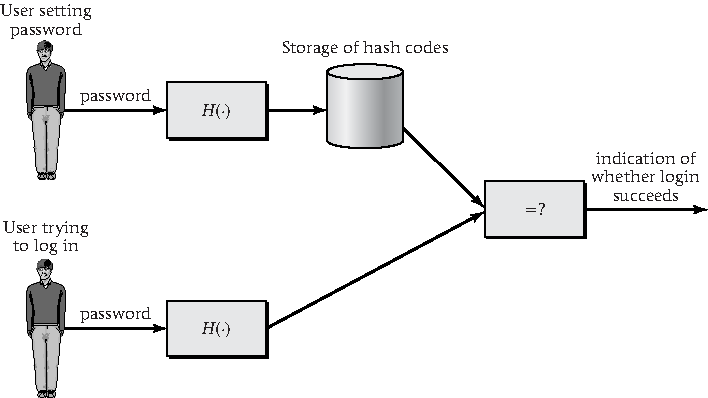
\includegraphics{hail_f1101}}
%\centerline{\def\epsfsize#1#2{0.6#1}\epsfbox{scan-11-1.eps}}
\caption{The system stores a
  cryptographic hash of the password when it is set, and compares that
  with the hash of the attempted password.  Because the hash function
  is collision-resistant, equal hashes mean the password was almost
  surely correct.  Because the hash function is difficult to invert,
  disclosure of the stored hash codes would not reveal the passwords.}
\label{scan-11-1}
\end{figure}
If the two hash codes are equal, then
for all practical purposes the system can be sure the correct password
was entered. However, if the stored hash values are disclosed, no one can
recover the passwords from them other than by trial and error.  One cost to user convenience is that the
system cannot support a function to ``remind me of my password,'' only
one to ``assign me a new password.''  In most settings, that is a
reasonable price to pay.

\subsection{Passwords for Multiple, Independent Systems}

In principle, you can easily avoid the problems stemming from using the
same password on multiple systems.  You just need to train yourself
not to pick the same password for shopping on Sleazy Sam's Super Saver
Site as you use to guard your employer's confidential records.  In
practice, however, picking a new password for every system would lead
to an unmemorizable array of different passwords.  Even one password
for each general category of system may be difficult.  Therefore, an
active area of development today is \foldvocab{password}{wallet}
systems, which store a range of passwords under the protection of one
master password.  The stored passwords constitute a security
vulnerability; this vulnerability is hopefully not so severe as the alternatives.

Another technique that can help users cope with multiple systems also
makes use of a master password but does not use it to protect storage
of individual passwords.  Instead, the individual passwords are
generated algorithmically from the master password and the sites'
names.  As an advantage compared with a password wallet, nothing at
all needs to be stored on the client machines.  As a disadvantage,
there is no easy way to change the master password.

\subsection{Two-Factor Authentication}\label{two-factor-section}

Even if a system is designed and operated so as to avoid the pitfalls
of spoofing, password storage, and password reuse, if it relies on
password-controlled login as its sole authentication method, it will
still possess the more fundamental vulnerabilities listed earlier.
Some of those can be overcome with sufficient user education or
mitigated in other ways.  For example, a system can be designed so as
to issue passwords (or pass phrases) that are random, and hence
difficult to guess, but are constructed out of real syllables or
words so as to be easily memorizable---an example of psychological acceptability.  To avoid problems with users
walking away, a system can demand reentry of the password before any
particularly sensitive operation or after any sufficiently long
period of inactivity.  All these countermeasures to password threats
are valuable but still leave something to be desired.  Thus, I will
turn now to other authentication methods.

Rather than relying on something the authorized user knows (a
password), an authentication mechanism can rely on something the user
physically possesses, such as a card or small plug-in device.  These
physical devices are generically called \vocabs{token}.  The big
problem with tokens is that they can be lost or stolen.  Therefore,
they are normally combined with passwords to provide
\foldvocab{two-factor}{authentication}, that is, authentication that
combines two different sources of information.  Another way to achieve
two-factor authentication is by combining either a password or a token
with \foldvocab{biometric}{authentication}, that is, the recognition
of some physical attribute of the user, such as a fingerprint or
retinal pattern.

The most familiar two-factor authentication system is that used for
bank automated teller machines (ATMs), in which you insert or swipe a card
and also type in a four-digit personal
identification number (PIN), which is essentially a short password.
Cards that use only magnetic stripes (as opposed to integrated circuits) are rather weak tokens, because they carry
fixed information rather than engaging in a cryptographic
authentication protocol and because they are easily copied.  However,
in the ATM application, they provide sufficient security that they continue to be used in the US.  In part,
this stems from other aspects of the system design, such as a limit on
how much money a customer can withdraw in a day.

One important difference between biometric authentication and other
techniques is that it is inextricably tied with actual human
identity.  A password-protected or token-protected account can be
issued to a person known only by a pseudonym, and it will never be
possible to ascertain the true identity of the user.  By contrast,
even if a biometric authentication user is initially enrolled without
presenting any proof of true identity (such as a passport), the user's
identity could later be deduced from matching the fingerprint (or
other biometric) with other records.  This is both an advantage and a
disadvantage.  Where the highest standards of accountability are
necessary, it can be advantageous.  However, it also cuts into
personal privacy.  For many purposes, pseudonymity is desirable, so
that people can dissociate some portion of their life from another
unrelated, perhaps earlier, portion.

When a user logs in using biometric authentication, some physical
device scans the user's fingerprint or other attribute and then
transmits a digitally coded version of the scan to a computer for
checking.  If an attacker can capture the digital version and later
replay it, the system's security will be breached, just as would be
the case if a password were captured and replayed.  One crucial
difference, however, is that a user can be issued a new password but
not a new fingerprint.  Therefore, the design of any biometric
authentication system needs to be particularly resistant to such
replay attacks.

Biometrics can be used for \vocab{identification} as well as
\vocab{authentication}. That is, a user's physical attributes can play
the role of a username (selecting a specific user) as well as of a
password (providing evidence that the selected user is actually
present).  However, biometric identification is a harder problem than
biometric authentication, as it requires searching an entire database
of biometric information, rather than only the information for a
specific user.  This broader search space increases the chance for
error.  Therefore, the most reliable systems still require the user to
enter some other identifier, such as a textual username.

\section{Access and Information-Flow
  Controls}\label{access-and-information-flow-controls-section}

In Chapter~\ref{processes-chapter}, I briefly made the distinction
between Discretionary Access Control (DAC), in which the creator or
other ``owner'' of an object can determine access rights to it, and
Mandatory Access Control (MAC), in which organizational policy directly
governs the access rights.  In that chapter, I then went into some
depth on capabilities and access control lists (ACLs), which are the two
mechanisms commonly used to implement DAC.  Therefore, I will now
focus on MAC in order to round out the picture.

The most well-developed MAC policies and mechanisms are geared to
protecting the confidentiality of information in national security
systems, where formal policies regarding the flow of information
predated the introduction of computer systems.  My discussion in this
section will be based on the policies of the United States government,
as is much of the published literature.  The general principles,
however, apply equally well to other similar systems of information
classification and user clearance.  In particular, after discussing
government classification systems, I will briefly remark on a
currently popular application to commercial web servers.  The goal
there is to limit the damage
if an attacker achieves control over the web server.

The United States military sponsored research, particularly in the
early 1970s, with the goal of allowing a single computer system to be
shared by principals operating on data of varying sensitivity and running
programs written by authors who are not fully trusted.  This sort of
system is known as a \vocab{Multi-Level Security} (\vocab{MLS})
system.  In this context, the technical security mechanism must
enforce \vocab{information-flow control} rather than only
\vocab{access control}.  That is, the system must protect sensitive
information from indirect disclosure rather than only from direct
access by unauthorized principals.

To appreciate the need for information-flow control in an MLS system,
consider the simplest possible system: one handling information of two
different levels of sensitivity.  Suppose objects containing high-level
information are labeled $H$ and those containing low-level (less
sensitive) information are labeled $L$.  There are some principals, those
with $H$ clearance, who may read and modify all objects.  There are
others, with $L$ clearance, who may only read $L$ objects.  So far,
access control would suffice, granting each class of principals access to
specific objects.  Now consider one further requirement: an
untrusted program run by an $H$ principal must not be allowed to copy
data out of an $H$ object and into an $L$ object where an $L$
principal could retrieve it.  Ideally, the program must also not leak
the information any other way, though as you will see, this is a
challenging requirement. I can summarize the requirements by saying
that information initially contained in an $H$ object must not flow to
an $L$ principal, even through means other than the $L$ user accessing
the object.

Real MLS systems handle more than two categories of information.  The
information is categorized in two ways.  First, there is an overall
\vocab{classification level}, indicating the degree to which disclosure could
damage national security.  In the United States, four classification levels are
used: unclassified, confidential, secret, and top secret.
(Technically, unclassified is not a classification level.  However, it
is handled like a level below the lowest true classification level, which is
confidential.) Second, there are \vocabs{compartment}, which indicate
topics, such as nuclear weapons or international terrorism.  A
principal may be cleared for access to data all the way up to top
secret classification, but be limited to a specific compartment, such as
nuclear weapons only.

Each object is labeled with exactly one
classification level  but can be
labeled with any set of compartments because (for example) a document
might concern the acquisition of nuclear weapons by international
terrorists.  Figure~\ref{scan-11-2} shows how each of the two kinds of
labels forms a partially ordered set, and Figure~\ref{scan-11-3}
shows how combining them results in another partially ordered set,
known mathematically as their Cartesian product.
\begin{figure}
\centerline{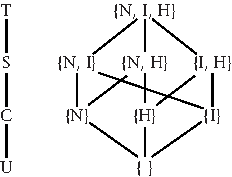
\includegraphics{hail_f1102}}
%\centerline{\def\epsfsize#1#2{0.6#1}\epsfbox{scan-11-2.eps}}
\caption{The classification levels top secret (T), secret (S),
  confidential (C), and unclassified (U) form a total order, as shown
  on the left.  Sets of compartments, on the other hand, form only a
  partial order, namely the subset order in which one set of
  compartments is below another if it has a subset of the other's
  compartments.  This is illustrated on the right with three
  hypothetical compartments: nuclear weapons (N), international
  terrorism (I), and human intelligence (H).  Someone cleared for
  $\lbrace \textrm{I}, \textrm{H} \rbrace$, for example, could read documents labeled
  with $\lbrace \textrm{I}, \textrm{H} \rbrace$, $\lbrace \textrm{I} \rbrace$, $\lbrace \textrm{H}
  \rbrace$, or $\lbrace \rbrace$.}
\label{scan-11-2}
\end{figure}
\begin{figure}
\centerline{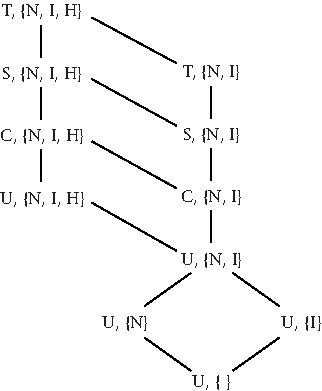
\includegraphics{hail_f1103}}
%\centerline{\def\epsfsize#1#2{0.6#1}\epsfbox{scan-11-3.eps}}
\caption{Forming the Cartesian product of the two partial orders from Figure~\ref{scan-11-2}
  results in a 32-element partial order, each element of which
  pairs one of the four classification levels (T, S, C, or U) with one of
  the eight sets of compartments (ranging from $\lbrace \textrm{N}, \textrm{I}, \textrm{H}
  \rbrace$ down to $\lbrace \rbrace$).  Of those 32 elements, only 11
  are shown here in order not to clutter the diagram.  What you should
  note in the diagram is the definition of ordering in the Cartesian
  product: a pair $(\textit{level}_1, \textit{compartments}_1)$
  dominates $(\textit{level}_2, \textit{compartments}_2)$ only if both
  $\textit{level}_1 \geq \textit{level}_2$ and
  $\textit{compartments}_1 \supseteq \textit{compartments}_2$.}
\label{scan-11-3}
\end{figure}

In a partial order, two elements may be ordered relative to one
another, with $x < y$ or $y < x$, or they may be unordered.  For
example, $\lbrace \textrm{I} \rbrace$ and $\lbrace \textrm{H} \rbrace$ are unordered,
because neither is a subset of the other.  In security applications, a
principal with clearance $p$ is allowed to view information with label
$i$ only if $p \geq i$, a condition known as $p$ dominating $i$ in the
partial order.  This rules out disclosing information to
principals with too low a clearance level, but also to those who
aren't cleared for all the necessary compartments.

Whenever an untrusted subject (that is, a process running an untrusted
program) has read from an object with label $l_1$
and then modifies an object with label $l_2$, an unauthorized
information flow may result unless $l_2 \geq l_1$.  That is,
information is only allowed to flow into an object whose consumers
could all have directly accessed the source information.  Strictly
speaking, the information flow results not from the
modification of an $l_2$ object {\em after} accessing the $l_1$
object, but rather from the modification of an $l_2$ object {\em based
on} the earlier access to the $l_1$ object.  However, it is extremely
difficult to test whether an earlier access has had some influence on
a later modification.  In particular, the earlier access can have a
subtle influence on whether the later modification occurs, as well as
an overt influence on the nature of that possible later modification.
Therefore, practical MLS systems generally take the simpler, more
conservative approach of forbidding any subject from modifying an
object that does not dominate all previously accessed objects in the
security label partial order.

The best-known information-flow control policy is known as the
\vocab{Bell-LaPadula model}, after the two MITRE Corporation
researchers who developed it in the early 1970s.\footnote{LaPadula's
  name was spelled La~Padula on the original publications and
  therefore is cited that way in the end-of-chapter notes and the
  bibliography.  However, in this section I will use the spelling
  LaPadula for consistency with most published descriptions, as well
  as with LaPadula's own current spelling of his name.}  The key idea
of the Bell-LaPadula model is to associate with each subject a current
level chosen by the principal running the subject process.  The
current level must be dominated by the principal's security clearance,
but can be lower in the partial order if the
principal chooses.  This
flexibility to run at a lower current level allows a principal to run
subjects that modify low-level objects and other subjects that read from
high-level objects, but not to have any one subject do both.  These
restrictions are enforced by two rules, each based on a formal
property from Bell and LaPadula's mathematical model, as follows:
\begin{itemize}
\item
A subject running with current level $c$ may read only from objects
with level $r$ such that $c$ dominates $r$, that is, $c \geq r$.  This
corresponds to Bell and LaPadula's \vocab{simple security property}.
\item
A subject running with current level $c$ may only modify an object
with level $m$ only if $m$ dominates $c$, that is, $m \geq c$.  This can be
derived from Bell and LaPadula's \vocab{*-property} (pronounced
\vocab{star-property}), which prevents untrusted programs from
transferring information into inappropriate objects.
\end{itemize}

In order for these two rules to effectively regulate information flow,
the Bell-LaPadula model also includes tight restrictions on how a
subject may change current levels.  In practical systems, the current
level is selected when a principal logs in and then is left unchanged
until the principal logs out.

You can gain some appreciate for the role of untrusted subjects in the
Bell-LaPadula model by considering that a principal may be
simultaneously logged in at two adjacent terminals, one set to a high
current level (as high as the principal is allowed) and the other set
to a low current level (unclassified, with no compartments).  The
human principal may display highly sensitive material on one terminal
and type it into an unclassified file on the other.  However, no
untrusted subject (that is, no process running an untrusted program)
may do the same information transfer.  The idea is that the human
principal is granted a high-level clearance only upon providing evidence
of trustworthiness.  Moreover, the principal can be monitored to
detect suspicious meetings, an excess of cash, and other signs of
corruption.  The author of the untrusted program, on the other hand,
is beyond reach of monitoring, and the group of low-clearance
principals who could be reading the leaked data is too large to
monitor.

Mandatory Access Control of the Bell-LaPadula variety can also be
combined with Discretionary Access Control using a mechanism such as
access control lists.  In fact, Bell and LaPadula themselves
recommended this.  The underlying security principle is \vocab{Need-To-Know}; that is, the possessor of sensitive information ought not to
disclose it to all principals of appropriately high clearance level,
but rather only to those with a specific need to know.  Compartments
provide a crude approximation to the Need-To-Know principle, but many
people cleared for a particular compartment will not have a
need to know any one specific document within that compartment.
Therefore, it is wise to give the owner of an object the ability to
further restrict access to it using an ACL.  However, unlike in a pure
DAC system, the ACL restrictions serve only to further refine the
access limits set by the simple security and *-properties.  An
otherwise cleared subject may be denied access for lack of an
appropriate ACL entry.  However, adding an ACL entry cannot grant
access to a subject running at an inappropriate current level.

Even with the Bell-LaPadula simple security and *-properties, an
untrusted subject may not be completely stopped from leaking sensitive
information.  Rather than leaking the information through a file,
network connection, or other legitimate storage or communication
object, the subject could disclose the sensitive information by way of
a \vocab{covert channel}.  A covert channel is a mechanism not
intended to be used for communication, but which can be manipulated by
one subject and observed by another, thus achieving communication.  An
example would be if a subject with access to highly sensitive
information varied the demands it placed on the CPU or disk based on
the sensitive information, and another subject, run at a lower
clearance level, was able to detect the changes in system utilization.
Complete protection against covert channels is impractical, but if
processes' resource utilization is tightly controlled, the risk can be
reduced.

Moving outside the area of military classification levels, one
currently popular MAC system is \vocab{Security-enhanced Linux}
(\vocab{SELinux}), a version of the Linux kernel.  This system is
quiet flexible and can enforce a wide variety of rules regarding
which objects each subject can read and write.  Objects are tagged
with type labels, which are a generalization of classification levels
and compartments.  Subjects are assigned to domains, which are a
generalization of clearance levels.  One popular configuration tags
the files containing web pages with a specific label and assigns the
Apache web server to a domain that is allowed to read those files but
not to write them nor to read any other files.  That way, even if an
attacker can exploit some bug in the web server to obtain control over
it and make it execute arbitrary code, it cannot leak confidential
information or damage the system's integrity.  This is an example of
the principle of least privilege.

\section{Viruses and Worms}\label{viruses-and-worms-section}

As the Bell-LaPadula model and SELinux illustrate, security mechanisms need to
limit the actions not only of users, but also of programs.  Limiting
programs' actions is important because they may be under the control
of untrusted programmers as well as because they may have exploitable
bugs that allow them to be misused.
In this section, I will address two
particular kinds of adversarial programs, or \vocab{malware}, that
pose especially widespread security threats.  The common feature of
viruses and worms, which distinguish these two kinds of malware from
garden-variety Trojan horses, is that one of the actions they are
programmed to take is to propagate themselves to other systems.  Thus,
an adversary can effectively attack all the computers on the Internet,
not by directly connecting to each one, but rather by attacking only a
few initial systems and programming each attacked system to similarly
attack others.  Through their sheer ubiquitousness, viruses and worms
constitute significant threats.

Both worms and viruses strive to replicate themselves.  The difference
is in how they do this.  A \vocab{virus} acts by modifying some
existing program, which the adversary hopes will be copied to other
systems and executed on them.  The modified program will then run the
inserted viral code as well as the original legitimate code.  The
viral code will further propagate itself to other programs on the
infected system as well as carrying out any other actions it has been
programmed to perform.  A \vocab{worm}, on the other hand, does not
modify existing programs.  Instead, it directly contacts a target
system and exploits some security vulnerability in order to transfer
a copy of itself and start the copy running.  Again, the worm can also
be programmed to take other actions beyond mere propagation.  Even
propagation alone can be a significant problem if carried out as fast
as possible, because the rapid propagation of worm copies can
constitute a denial-of-service attack.

Viruses were a greater problem in the days when the major
communication channel between personal computers was hand-carried
diskettes.  As the Internet has become dominant, worms have become the
more common form of self-propagating malware.  However, because of the
earlier prominence of viruses, many people inaccurately use the word
virus to refer to worms.

Any network-accessible vulnerability that a human intruder could
exploit can in principle be exploited by a worm in order to
propagate.  Historically, for example, worms have used password
guessing.  Also, as mentioned in Chapter~\ref{processes-chapter},
email worms are common today; these worms arrive as email
attachments and are run by unwary users.  However, the most serious
means of worm propagation has come to be the exploitation of
buffer-overflow vulnerabilities.  Therefore, I will explain this
common chink in systems' defenses.

Most programs read input into a contiguous block of virtual memory,
known as a buffer.  The first byte of input goes into the first byte
of the buffer, the second into the second, and so forth.  Often, the
program allocates a fixed-size buffer rather than allocating
progressively larger ones as more and more input arrives.  In this
case, the programmer must test the amount of input against the size of
the buffer and take some defensive action if an unreasonably large
amount of input is presented, which would otherwise overflow the
buffer.  Unfortunately, programmers perennially omit this
checking. Therefore, adversaries are perennially able to find programs
that, when presented with unusually large inputs, try to write the
input data into addresses beyond the end of the buffer.  This is
particularly problematic for network server programs, which can be
provided input by an adversary elsewhere on the Internet.

The consequences of a buffer overflow depend heavily on the
programming language implementation, operating system, and computer
architecture.  In modern languages such as Java, any attempt to write
past the end of an array is detected.  Often, the detected error will
cause the attacked server program to crash.  In some cases, this is
victory enough for an adversary.  However, it is minor compared with
the damage an adversary can do when exploiting a buffer overflow in a
program written using more primitive technology, such as typical
implementations of the programming language C.  In those settings, the
extra input data may be written to addresses beyond the end of the
buffer, overwriting other data assigned to those later addresses.

One possible tactic an adversary could use is to look for a server
program in which a buffer is followed by some particularly sensitive
variable, such as a Boolean flag indicating whether a password has
been successfully checked yet.  However, buffer-overflow exploits
typically take a different approach, which allows the adversary 
to inject entirely new instructions for the process to execute, which
it ordinarily would not even contain.  In this way, the server process
can be made to take any action whatsoever, within the limits of the
authority it has been granted.  This an extreme example of
misalignment between authority and control.

To understand how a buffer overflow can lead to the execution of
arbitrary code, you need to consider some facts about typical runtime
stacks, which are described in Appendix~\ref{stacks-appendix}.  Often, program
variables such as buffers are allocated their space within the stack.
The stack also typically contains the return address for each
procedure invocation, that is, the address of the instruction that
should be executed next when the procedure invocation returns.  If the
stack grows downward in virtual memory, expanding from higher
addresses down into lower ones, then the return address will follow
the buffer, as shown in Figure~\ref{stack-smashing}(a).

In this circumstance, which arises on many popular
architectures, a buffer overflow not only can overwrite data values,
as shown in Figure~\ref{stack-smashing}(b), but also can overwrite the
return address, as shown in Figure~\ref{stack-smashing}(c).  This form
of buffer overflow is commonly called \vocab{smashing the stack}.
\begin{figure}
\centerline{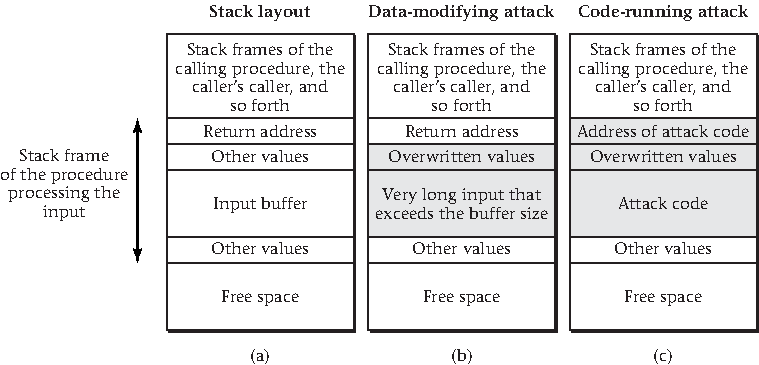
\includegraphics{hail_f1104}}
%\centerline{\def\epsfsize#1#2{0.6#1}\epsfbox{stack-smashing.eps}}
\caption{If input (shown in grey) is allowed to overflow the amount of memory
  allocated on the stack for an input buffer, it can overwrite other
  data values, as shown in part (b), or the return address, as shown
  in part (c).  In the latter case, the modified return address can point to
  attack code included in the oversized input.}
\label{stack-smashing}
\end{figure}
When the current procedure invocation completes, the overwritten
return address causes the processor to jump to an adversary-specified instruction
address.  On its own,
this would allow the adversary only to choose which existing code to
execute.  However, when taken together with one other factor, it
provides the means to execute code provided by the adversary.

Many architectures and operating systems provide virtual memory
mechanisms that allow each page of virtual memory to be independently
read-protected or write-protected, but that do not allow a
distinction between reading data and fetching instructions.  In this
circumstance, the pages holding the stack, which need to be readable
for data, can also contain executable code---even though extremely few
programs legitimately write instructions into the stack and then jump
to them.

An adversary can exploit this situation by writing a large input that
not only overflows the buffer and overwrites the return address, but
also contains the bytes constituting the adversary's choice of machine
language instructions.  These machine language instructions 
are labeled as attack code in Figure~\ref{stack-smashing}(c).  The overwritten return address is used to jump
into the buffer itself, thereby executing the provided instructions.

Because these exploits are so prevalent, there has been considerable
interest recently in modifying virtual memory mechanisms so as to
allow stack space to be readable (and writable) but not executable.
Other than techniques such as this for preventing malware from
entering, the major countermeasure has been the use of antivirus
scanning programs, which commonly scan for worms as well.  These
programs look for distinctive patterns of bytes, known as
\vocabs{signature}, found in known viruses and worms.  As such,
scanners need to be frequently updated with signatures for newly
emerging threats.

\section{Security Assurance}\label{security-assurance-section}

Organizations directly influence their systems' security through the
manner in which the systems are installed and operated, as well as through
the design of components developed in-house.  However, the
organizations also exercise more indirect control by choosing to
procure security-critical components from vendors that demonstrate
that the components are suited to the organizations' needs.  In this
section, I will explain how this kind of security assurance is
provided by vendors and interpreted by consumers.  The component in
question may be an operating system, middleware system, or a network
device such as a firewall or intrusion detection system, among
others.  In the security assurance field, any of these may be referred
to as a \vocab{Target of Evaluation} (\vocab{TOE}), because the
assurance derives from an independent evaluation of how well the TOE
satisfies stated security requirements.

The assurance of security-related products is governed by an
international standard called the \vocab{Common Criteria}, because it
was developed to harmonize previously independent national standards.
The Common Criteria are also sometimes known by their International
Standards Organization number, ISO~15408.  The Common Criteria define
a process in which a vendor contracts with a qualified independent
assessor to evaluate how well a product meets a set of security
requirements known as a \vocab{Security Target} (\vocab{ST}).

Each ST is an individual requirements document specific to the
particular product under evaluation, that is, specific to the TOE.  However,
because consumers can more easily  compare products whose STs
share a common basis, the STs are built in a modular fashion from
common groups of requirements.  A published group of requirements,
intended to be used as the basis for multiple STs, is called a
\vocab{Protection Profile} (\vocab{PP}).

Just as STs are built from standard PPs, each PP is assembled by
choosing from a standard menu of potential requirements.  Extra custom
requirements can be added at either stage, but the bulk of any ST's
requirements will come from the standard list by way of one of the
standard PPs.  Thus, consumers are in a better position to learn their
way around the landscape of potential requirements.  This is critical,
because a product certified by an independent assessor to meet its ST
is worthless if that ST does not contain requirements appropriate to a
particular consumer's needs.

The requirements contained in PPs and STs fall into two general
categories: functional requirements and assurance requirements.  An
example of a functional requirement would be a mandate for a
spoofing-resistant login method. (Microsoft Windows would satisfy this
requirement, using CTRL+ALT+DEL.)  An example of an assurance
requirement would be a mandate that detailed design documents, testing
reports, and samples of security-critical code be reviewed by outside
evaluators.

The assurance requirements are summarized by a numerical
\vocab{Evaluation Assurance Level} (\vocab{EAL}), in the range from
EAL1 to EAL7.  For example, an ST based on EAL4 will contain
moderately rigorous demands regarding the evidence that the system
actually meets its functional requirements, but none that go beyond
ordinary good development practices outside the security field.  At
EAL5 and above, specific security-oriented assurance practices need to
be incorporated into the development process, including progressively
increasing use of semiformal and formal methods.
Figure~\ref{EAL-figure} gives a brief rubric for each EAL, taken from
\begin{figure}
\centerline{\begin{tabular}{|l|l|}
\hline
\bf EAL & \bf Rubric \\\hline
EAL1 & functionally tested\\
EAL2 & structurally tested\\
EAL3 & methodically tested and checked\\
EAL4 & methodically designed, tested, and reviewed\\
EAL5 & semiformally designed and tested\\
EAL6 & semiformally verified design and tested\\
EAL7 & formally verified design and tested\\\hline
\end{tabular}}
\caption{This table shows brief rubrics for the Common Criteria Evaluation Assurance
  Levels; expanded descriptions are available in the Common Criteria documentation.}
\label{EAL-figure}
\end{figure}
the Common Criteria documentation.

Although each EAL includes a whole package of sophisticated assurance
requirements, the EALs can be easily understood in a comparative way:
a higher-numbered EAL is stricter.  This makes it tempting to focus on
the EALs.  However, you need to remember that an EAL, even a very
strict one, tells only how thorough a job the vendor has done of
demonstrating that the TOE meets the functional requirements that are
in the ST.  It tells nothing about how demanding those functional
requirements are.  More importantly, the EAL tell nothing about how
well matched the requirements are to your needs.

As an example, Microsoft contracted for a Common Criteria evaluation
of one particular version of Windows, relative to an ST that included
the assumption that the only network connections would be to equally
secure systems under the same management and that all authorized
users would be cooperative rather than adversarial.  Thus, it gave no
indication how well the system would fare if confronted with serious
adversaries, either within the user population or out on the Internet.
These issues arise from the functional requirements in the ST,
completely independent of the EAL.  Figure~\ref{windows-st} shows the
relevant language from Microsoft's ST.
\begin{figure}
\centerline{\fbox{\parbox{25pc}{
\begin{itemize}
\item
Any other systems with which the TOE communicates are assumed to be
under the same management control and operate under the same security
policy constraints.  The TOE is applicable to networked or distributed
environments only if the entire network operates under the same
constraints and resides within a single management domain.  There are
no security requirements that address the need to trust external
systems or the communications links to such systems.
\item
Authorized users possess the necessary authorization to access at
least some of the information management [sic] by the TOE and are
expected to act in a cooperating manner in a benign environment.
\end{itemize}\vspace*{-1em}}}}
\caption{These excerpts are from the Windows 2000 Security Target, ST Version
  2.0, 18 October 2002, prepared for Microsoft Corporation by Science
  Applications International Corporation.}
\label{windows-st}
\end{figure}

The weakness of these small excerpts from one particular ST may leave
you wondering about the value of the Common Criteria process.  The
lesson you should take away is not that the Common Criteria process is
worthless, but rather that it relies upon educated consumers.  To
benefit from the process, you need to understand its vocabulary, such
as what the difference is between an EAL and an ST.

\section{Security Monitoring}\label{security-monitoring-section}

System operators have at least three reasons to monitor for attacks,
both successful and unsuccessful:
\begin{itemize}
\item
By gaining a better understanding of adversaries' behavior, you can
develop better countermeasures.
\item
By putting adversaries on notice that you may gather enough evidence
to allow successful prosecution or other punishment, you may deter
attacks.  This tends to work better against adversaries within your
organization than against adversaries on the other side of the
Internet.  You should coordinate in advance with legal counsel on
appropriate policies and notices.
\item
By quickly detecting a successful attack, you can limit the damage, and
by obtaining accurate information about the extent of the damage, you
can avoid overly conservative responses, such as reinstalling software
on uncompromised systems.  Overly conservative responses not only take
time and money, they also require system downtime.  Thus, an overly
conservative response magnifies the damage done by an attack.
\end{itemize}

For all these reasons, security professionals have been very active in
developing monitoring techniques.  I already mentioned one in
Chapter~\ref{networking-chapter}, namely network intrusion detection
systems (IDSes).  Others that I will summarize here include robust
logging facilities, integrity checking software, and honeypots.

Intrusion detection systems are perhaps best thought of as anomaly
detectors for network traffic.  Many IDSes can be configured to spot
anomalous traffic even if it results from an adversary internal to
your network, rather than an intruder.  Thus, the name IDS is somewhat
misleading.  An IDS may look for specific attack signatures or may
respond to deviations from past patterns of activity.  For example, if
a normally quiet desktop machine starts spewing out UDP datagrams at the
maximum rate the network can carry (as it would if infected with the
SQL Slammer worm), even an IDS that had no signature for the specific
worm ought to raise a warning about the sudden traffic.

Other anomalous events may be detected internal to a particular
system, rather than in network traffic.  For example, an operating
system may be programmed to note repeated failed attempts to log in as
the system administrator, which could constitute a particularly
dangerous password-guessing attack, worthy of notice even if
unsuccessful.  These sorts of anomalies are routinely logged by systems
into a chronological event log, which can be used to reconstruct a
break-in after the fact as well as serving as a source to drive
real-time alerts.  The biggest technical challenge is that a
successful attack may give the adversary the necessary access privileges
to clean up the log, covering traces of the attack.  High-security
systems therefore use append-only logging devices.  Log entries can
also be sent over the network to a centralized, heavily-protected
logging server.

Another non-network monitoring approach is to periodically check the
integrity of a system's configuration, such as whether any of the
system programs have been modified.  Successful attackers will
frequently modify programs or configuration files so as to give
themselves a \vocab{back door}, that is, a second way in to use even
if the initial vulnerability is fixed.  Thus, a periodic check may
turn up signs of a successful break-in since the previous check,
even if the break-in was sufficiently stealthy to otherwise go unnoticed.

In addition to periodic checks, the same integrity checking can be
done after any break-in that comes to notice through other means.
Without integrity checking, a system administrator has little choice
but to treat the whole system as compromised, scrub it clean, and
reinstall from scratch.  Thus, integrity checking not only allows
successful attacks to be detected, it also guides the mounting of an
appropriate response.

An example integrity monitoring system is \vocab{Tripwire}.  The basic
principle of operation is that a cryptographic hash of each critical
file is computed and stored in a tamper-resistant database, such as on
a CD that is writable only once.  The Tripwire program itself is also
stored in tamper-resistant form.  To check the system, the known-good
copy of Tripwire recomputes the cryptographic hashes and compares them
with the stored copies.

The integrity checking needs to be done with a tamper-resistant program
because
attackers frequently install modified versions of system programs
that hide the corruption.  For example, the attacker may install a version
of \verb|ps| that hides the attacker's processes and a version of \verb|ls|
that shows the \verb|ps| and \verb|ls| programs as though they were unmodified.
This kind of camouflage is commonly called a \vocab{root kit}.

The final form of security monitoring I will mention is the use of
honeypots.  A \vocab{honeypot} is a decoy system used specifically to
monitor adversaries.  It is configured to appear as realistic as
possible but is not used for any genuinely valuable purpose other than
monitoring.  It is subject to extreme but clandestine monitoring, so
as to fully record adversaries' behavior but not tip them off.
Because no legitimate user will ever have reason to connect to the
honeypot, the monitoring can be comprehensive---no anomaly detection
filtering is needed to distinguish legitimate traffic from attack
traffic.

By letting an adversary take over the system, rather than immediately
repelling the attack, you can learn more about the attack techniques
beyond the initial connection and thus learn more about
vulnerabilities you need to repair on other systems, as well as other
countermeasures you need to take.  However, because the adversary is
allowed to take over the honeypot, it must be thoroughly firewalled
against outbound attacks so that you don't provide the means to
launch attacks on further systems.  Humans should also monitor the
honeypot continuously and be ready to intervene.  These considerations
help explain why honeypots, although quite in vogue, are best left to
large organizations with experienced security professionals.  Smaller
organizations can still benefit because honeypots largely provide
epidemiological evidence about what worms are circulating, which can serve
the whole Internet community.

\section{Key Security Best
  Practices}\label{key-security-best-practices-section}

Appropriate security practices depend on many factors, including
whether you are defending your home computer or an employer's
high-value system and whether you are engaging in custom
application-software development or only procuring, installing,
configuring, and operating existing systems.  However, I will attempt
a unified list of best practices with the understanding that some may
be more applicable than others to any one context:
\begin{itemize}
\item
Consult others.  Everybody, even home users, should at least read the
the website of the \index{SANS}SANS (SysAdmin, Audit, Network,
Security) Institute, \textit{\url{http://www.sans.org}}.  Organizations should also hire reputable
consultants, as well as engage in conversations with legal counsel,
those responsible for noncomputer security, and the human resources
department.
\item
Adopt a holistic risk-management perspective.  Consider how much you
have to lose and how much an adversary has to gain, as well as how
likely an adversary is to be caught and punished.  Are any of these
factors more manipulable than the inherent vulnerability of your
system?
\item
Deploy firewalls and make sure they are correctly configured.  The
best approach combines hardware firewalls guarding organizational and
workgroup perimeters with software firewalls guarding individual
machines.  Even a home can use this approach, often with a NAT router
serving as the hardware firewall.
\item
Deploy anti-virus software.  An organization should have server-based
software that scans all incoming email so as not to be at risk should
an individual client machine fail to scan.  However, the individual
client machines should also have protection for defense in depth and
in particular to guard against infections that sneak past the network
perimeter by being carried in on a portable computer or storage
device.
\item
Keep all your software up to date.  This includes not
only system software such as the operating system, but also any
application software that may be exposed to data from the network.
Today, that includes nearly everything.
\item
Deploy an IDS, integrity checking software such as Tripwire, and a
robust logging platform.  These steps are not very practical for
typical home users yet.
\item
Assume all network communications are vulnerable; use end-to-end
encryption rather than relying on the security of network
infrastructure.  The same principle applies if storage media are
physically shipped between locations.
\item
Use two-factor user authentication, as described in
Section~\ref{two-factor-section}.
\item
Maintain physical security over computer equipment and be vigilant of
service personnel or others with extraordinary physical access.
\item
Do what you can to stay on good terms with employees and to part from
them cleanly.  When hiring for particularly sensitive positions, such
as system administrators, candidly disclose that you will be checking
background and do so.  Establish realistic expectations that do not
encourage people to work nights or weekends when no one else is
around.  Have employees cross-train one another and take vacations.
\item
Establish and clearly communicate policies on acceptable use and on
monitoring.
\item
Beware of any security-relevant phone calls and emails that you do not
originate, as well as of storage media that arrive by mail or courier.  A
``vendor'' with a critical patch you need to install could be a con
artist.  The same is true of a law-enforcement agent or a member of
your organization's upper management; being cooperative should not
preclude taking a minute to politely confirm identity and authority.
\item
Examine closely any case where the user whose authority is exercised by a process is not the same as the user who controls the process's actions:
\begin{itemize}
\item
If at all possible, never run a program from an untrusted source.
Failing that, run it with the least possible authority and the
greatest possible monitoring.
\item
If you need to write a setuid program, check very carefully what it
does with all user input.  Might any buffer overflow?  Might any input
be interpolated into a shell command or otherwise allowed to exert
control?  Did a programmer insert an intentional ``trapdoor,'' whereby
a particular input can trigger the program to bypass normal security
controls?  Are there any TOCTTOU races?  Also, have the program owned
by a special-purpose user account that is granted only the necessary
authority.  More generally, review the principles listed in
Section~\ref{security-objectives-and-principles-section}.
\item
Examine any program that communicates over the network according to the
exact same standards as a setuid program.
\end{itemize}
\end{itemize}

\section*{Exercises}
\begin{chapterEnumerate}
\item
To keep certain individuals from flying on commercial airliners, a
list is maintained that airlines must check before issuing a
boarding pass.  The pass may be issued over the web, as well as at the
airport.  The pass must be presented to a human at the airport along
with an identifying document.  The human, who uses no computer
technology, checks that the name on the pass matches that on the
identifying document and that the photo on the identifying document
matches the appearance of the person presenting it.  This check is
done at the perimeter of the secured portion of the airport as an
admission condition.  You may assume that identifying documents are
hard to forge and that getting past the perimeter control without
going through the check is difficult.
\begin{enumerate}
\item
How could an adversary get admitted to the secure area despite being
on the no-fly list?
\item
Is the vulnerability you identified in part (a) one that could be
explained by inattention to any of the security principles listed in
Section~\ref{security-objectives-and-principles-section}?
\item
Can you design a countermeasure to deter the exploitation of the
vulnerability you identified?  Would the use of additional computer
technology help you do so without sacrificing desirable properties of
the current system?
\end{enumerate}

\item
An organization's checks are preprinted with a statement that checks
for \$100 or more require a handwritten signature, whereas smaller
checks are valid with a printed signature.  How is this explainable in
terms of the general principles of security enumerated in
Section~\ref{security-objectives-and-principles-section}?

\item
Section~\ref{security-objectives-and-principles-section} contains a
long list of general security principles.  For each of the following
audiences, suppose you had time to explain only a few of the
principles.  Which few would you explain?  Why?
\begin{enumerate}
\item software developers designing and programming new systems
\item information technology staff who will be
  purchasing, configuring, and administering systems
\item the Chief Information Officer, who is the executive supervising both of
   the above groups
\end{enumerate}

\item
Another weakness of password security is that there is always an administrator
to whom a user can turn upon forgetting a password.  That administrator has the ability
to reset the password.  This person may be gulled by a con artist (who
tells a pitiful tale of woe) into resetting a password without first
authenticating the user in some alternate manner, for example, by using a
photograph on an ID card.
\begin{enumerate}
\item
What is the name for the general category of threat of which this is
an example?
\item
Even if the human customer-service staff can't be stopped from
resetting passwords like this, the system can be programmed to print
out a letter acknowledging the password change, which is mailed by
ordinary postal mail to the registered address of the user.  Why would
this enhance security, even though it wouldn't prevent the adversary
from obtaining access?
\end{enumerate}

\item
What is two-factor authentication?  Give an example.

\item
Why should a blank web form to be filled in with a password be
downloaded to the browser via SSL, rather than using SSL only to send
the filled-in form back to the server?

\item
Draw the following partially ordered sets:
\begin{enumerate}
\item
One based on the subset ordering for sets of compartments, as in
Figure~\ref{scan-11-2} on page~\pageref{scan-11-2}, but using only the N and I compartments.
\item
The full Cartesian product of your answer from part (a) and the total
ordering of $\lbrace \textrm{T}, \textrm{S}, \textrm{C}, \textrm{U} \rbrace$.  Unlike
Figure~\ref{scan-11-3} on page~\pageref{scan-11-3}, no elements should be left out.
\end{enumerate}

\item
Figure~\ref{cartesian-product-skeleton} shows the full 32-element
Cartesian product of the 4-element and 8-element partial orders shown
in Figure~\ref{scan-11-2} on page~\pageref{scan-11-2}.  However, the
elements are not labeled with their security classification levels and
sets of compartments; instead, they are shown just as circles.  What
should the labels be for the eight circles shown in black?  (Note that
this diagram is arranged differently than the 11-element excerpt in
Figure~\ref{scan-11-3} on page~\pageref{scan-11-3}.  Do not expect to
find those 11 elements in the same positions here.)
\begin{figure}
\centerline{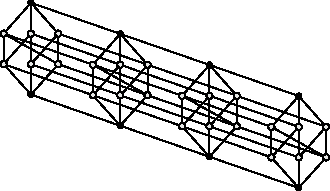
\includegraphics{hail_f1107}}
%\centerline{\def\epsfsize#1#2{0.6#1}\epsfbox{cartesian-product-skeleton.eps}}
\caption{This is an unlabeled version of the Cartesian product of the partial
  orders shown in Figure~\ref{scan-11-2} on page~\pageref{scan-11-2}.}
\label{cartesian-product-skeleton}
\end{figure}

\item
Using the Bell-LaPadula model, with the compartments $\lbrace \textrm{N}, \textrm{I}, \textrm{H}
\rbrace$ and classification levels $\lbrace \textrm{T}, \textrm{S}, \textrm{C}, \textrm{U} \rbrace$, which of
the following statements are true?
\begin{enumerate}
\item
A subject with current level C and compartments N and H may
read from an object with level C and compartments N and H.
\item
A subject with current level C and compartments N and H may
read from an object with level C and compartment N.
\item
A subject with current level C and compartments N and H may
read from an object with level C and compartments N, I, and H.
\item
A subject with current level C and compartments N and H may
read from an object with level C and compartments N and  I.
\item
A subject with current level C and compartments N and H may
read from an object with level S and compartments N and H.
\item
A subject with current level C and compartments N and H may
read from an object with level S and compartment N.
\item
A subject with current level C and compartments N and H may
read from an object with level S and compartments N, I, and H.
\item
A subject with current level C and compartments N and H may
read from an object with level U and no compartments.
\item
A subject with current level C and compartments N and H may
write into an object with level C and compartments N and H.
\item
A subject with current level C and compartments N and H may
write into an object with level C and compartment N.
\item
A subject with current level C and compartments N and H may
write into an object with level C and compartments N, I, and H.
\item
A subject with current level C and compartments N and H may
write into an object with level C and compartments N and  I.
\item
A subject with current level C and compartments N and H may
write into an object with level S and compartments N and H.
\item
A subject with current level C and compartments N and H may
write into an object with level S and compartment N.
\item
A subject with current level C and compartments N and H may
write into an object with level S and compartments N, I, and H.
\item
A subject with current level C and compartments N and H may
write into an object with level U and no compartments.
\end{enumerate}

\item
In the Bell-LaPadula model, under what conditions may a subject read
from an object and then modify the object to contain new information
that is derived from the old?

\item
Why, in the Bell-LaPadula model, is it important that a principal can
run a subject at a current security level below the one the principal
is cleared for?

\item
In the Bell-LaPadula model, a subject running at a high current level
may read from an object that is labeled with a lower level.  In a
system with readers-writers locks, this could block a subject running
at a lower level from writing the object.  Explain why this could
compromise the design goals of the Bell-LaPadula model.

\item
Viruses have historically been a problem primarily on systems designed
with little regard for the principle of least privilege.  Explain why
this would be expected.  Keep in mind the distinction between viruses
and worms.

\item
A Common Criteria assessment includes inspection not only of the
system design and code, but also of documentation intended for system
administrators and users.  Why is this relevant?

\item
Explain the difference in the Common Criteria between a PP, an ST, and
an EAL.

\item
Is a system certified at a high EAL necessarily more secure than one
certified at a low EAL?  Explain.

\item
Distinguish honeypots from IDSes.

\item
Why should the code of network server programs be audited for correct
processing of received input in the same way a setuid program's
processing of user input is audited?

\item
Section~\ref{user-authentication-section} points out that password-based user authentication is vulnerable to a user walking away and being replaced at the keyboard by an adversary.  Section~\ref{two-factor-section} indicates that this vulnerability can be mitigated, but not eliminated, by demanding reentry of the password at appropriate moments.
\begin{enumerate}
\item
Explain how the vulnerability might be more thoroughly mitigated using an appropriately designed token.
\item
Explain how the vulnerability might be eliminated using biometric authentication.
\end{enumerate}

\end{chapterEnumerate}

\section*{Programming Projects}

\begin{chapterEnumerate}

\item
Write a program that runs all strings of six or fewer lowercase
letters through a library implementation of SHA-1.  Report how long
your program takes, with enough details of the hardware and software
context that someone could approximately replicate your result.

Consider the system shown in Figure~\ref{scan-11-1} on
page~\pageref{scan-11-1} in which the hash function can be SHA-1.
The point of this system is to increase an adversary's work factor if
the stored value is disclosed.  Based on your experiment, you should
have some indication how much the work factor increases by, given an
assumption that users pick passwords of the sort your program
checked.  Under what sorts of circumstances would this increase in
work factor be sufficient?

\item

On a Linux system, you can read cryptographically-strong random bytes
from {\tt /dev/random} and can generally read a list of words (one
per line) from a file such as {\tt /usr/share/dict/words}.
Other systems are likely to have similar information available.  Write
a program that randomly chooses four words, each of which is four
letters long, and prints them
out with hyphens between them to serve as a passphrase.  For
example, you might get the output {\tt mean-chef-pour-pubs}.  On the
Linux distribution on my computer, there are 2236 four-letter
words.  How many four-word passphrases can be formed from them?  How
long would a random string of lowercase letters need to be to have a
comparable number of possibilities?  Which seems to be more memorizable?

\end{chapterEnumerate}

\section*{Exploration Projects}
\begin{chapterEnumerate}

\item\label{paris-hilton-project}
User authentication systems are successfully attacked all the time,
usually without generating much publicity.  However, when the user in
question is a celebrity, the newspapers sit up and take notice.  Write
a summary of a user-authentication failure involving Paris Hilton in
February of 2005.  Your sources should include at least the article that
month by Brian McWilliams in \textit{MacDev Center} as well as the
article by Brian Krebs in the May 19, 2005, issue
of \textit{The Washington Post}; both articles are cited in the
end-of-chapter notes.  As these articles contain contradictory
information, presumably they should be taken with a grain of salt.
Nonetheless, are there any lessons you can draw, both for designers of authentication systems and
for users?

\item
The website \textit{\url{http://www.sans.org}} contains a list of top-twenty vulnerabilities.  Look at the information
given on how to remedy each problem.  How many of these correspond to
the best practices listed in this chapter?

\item
Research and write a paper about the role that Trojan horses
reportedly played in a 2004 unauthorized access to Cisco Systems and
in a 2005 unauthorized access to LexisNexis's Seisint unit.  In the
first, the Trojan horse was reportedly a version of the {\tt ssh}
program, whereas in the second, the Trojan horse reportedly
masqueraded as a display of nude photos of a teenage girl.  Setting
that difference aside, what commonality and what other differences can
you find in the way the two attacks worked?  What more general lessons
for computer system security can be gained from these two incidents?

\item
Most UNIX and Linux systems include a program called {\tt sudo}.  Read
the documentation for it on your system or on the web at
\textit{\url{http://www.sudo.ws}}.  Write a description of how this
program's design reflects several of the principles explained
in this chapter.

\item
Check the web sites of a variety of banks to see whether they have login forms available through http (non-SSL) URLs, rather than only https (SSL-encrypted) ones.  Document your findings using screen captures.

\item
Find several commercially available biometric systems.  For each one, indicate whether it provides identification or only authentication.

\item
What is address space layout randomization and how does it help deter stack smashing attacks?

\item
Bradley Manning has been charged with disclosing a large volume of classified information to WikiLeaks. Write a paper that uses
publicly available information about this case to illustrate general security principles.

\end{chapterEnumerate}

\section*{Notes}

The single most important source of practical information about
security is \index{SANS}\textit{\url{http://www.sans.org}}.  There
are also a number of good books on practical security matters, such as
those by \index{Garfinkel, Simson}Garfinkel, \index{Spafford, Gene}Spafford, and \index{Schwartz, Alan}Schwartz~\cite{max1166}; \index{Cheswick, William R.}Cheswick,
\index{Bellovin, Steven M.}Bellovin, and \index{Rubin, Aviel D.}Rubin~\cite{max1165}; and \index{Northcutt, Stephen}Northcutt et
  al.~\cite{max1167}.  For a broad treatment of security,
\index{Anderson, Ross}Anderson's book~\cite{max1195} is highly regarded.

\index{Saltzer, Jerome H.}Saltzer and \index{Schroeder, Michael D.}Schroeder presented most of Section~\ref{security-objectives-and-principles-section}'s general security
principles in their 1975 tutorial paper~\cite{max1164}.  That
paper also described capabilities and access control lists, along the
lines of Chapter~\ref{processes-chapter}'s presentation.

Because one important class of security threats involves tricking legitimate users
into cooperating with an adversary, \index{Stajano, Frank}Stajano and \index{Wilson, Paul}Wilson have analyzed the methods
that con artists use~\cite{max1196,max1197}.

One example of a system that generates multiple passwords from a
single master password was described by \index{Ross, Blake}Ross et al.~\cite{max1178}.

The Bell-LaPadula model was described by \index{Bell, D. E.}Bell and \index{La Padula, L. J.}La~Padula in a
series of MITRE Corporation technical reports in the early 1970s.
Their best summary is in a later ``unified exposition,'' which was
also published only as a technical report~\cite{max1158}.  A more
sophisticated, but less influential, information-flow model was
published by \index{Denning, Dorothy E.}Dorothy Denning~\cite{max1037}. Both of these and other
formal models were surveyed by \index{Landwehr, Carl E.}Landwehr~\cite{max1038}.  The problem
of covert channels was described by \index{Lampson, Butler W.}Lampson~\cite{max1159}.  Another
important survey of the state of security research in the
highly-productive 1970s was published by \index{Denning, Dorothy E.}Dorothy and \index{Denning, Peter J.}Peter
Denning~\cite{max1046}.

I mentioned that although most buffer-overflow attacks overwrite
return addresses, an attacker could instead arrange to overwrite some
security-critical variable, such as a Boolean flag used to control
access.  \index{Chen, Shuo}Chen et al.~\cite{max1176} showed that such attacks are in
fact realistic, even if not currently popular.  As defenses are put in
place against current-generation stack-smashing attacks, these
alternate forms of attack are likely to gain in popularity.

Information about the \index{Common Criteria}Common Criteria is available from
\textit{\url{http://www.commoncriteriaportal.org}}.  A good overview is in the introductory
document~\cite{max1161}.  The specific ST that I use for illustration
is the one for Windows 2000~\cite{max1160}.  It was also used by
\index{Shapiro, Jonathan S.}Shapiro to make similar points about the importance of functional
requirements~\cite{max1163}.

Exploration Project~\ref{paris-hilton-project} mentions a user
authentication failure involving \index{Hilton, Paris}Paris Hilton.  Many published
accounts at the time included some information about the attack; the
one specifically mentioned in the project assignment is by
\index{McWilliams, Brian}McWilliams~\cite{max1162}.  Information about the attack seems to have shifted over time;
the project assignment also mentions an article a few months later by
\index{Krebs, Brian}Krebs~\cite{max1177}.
